\documentclass[a4paper,twoside,DIV15,BCOR12mm]{scrbook}

%exam will consist of 2-4 excercises, 1h wiht 60 points meaning 1min for 1 point
%per exercie there a 2 - 4 part
%discuss paper, extend design, how to improve, report main questions, main designs, etc.

\usepackage{Econ}

%standard setup
\author{Prof. Dr. Nora Szech}
\publishers{Martin Belica}
\title{Economics and Behaviour}
\date{Wintersemester 2015}

%latexki
\author{Prof. Dr. Nora Szech}
\semester{Wintersemester 2015}
\scriptstate{work-in-progress}

\makeindex

\begin{document}

\pagenumbering{arabic}
\setcounter{page}{1}

%!TEX root = Funktionalanalysis - Vorlesung.tex

\maketitle
%!TEX root = Funktionalanalysis - Vorlesung.tex


\chapter*{Preface}
This \textbf{unofficial} script has been created by Martin Belica in WS 2015/16 containing notes from the lectures by Prof.~Dr.~Szech at the KIT. This is an extended version, meaning it contains additional definitions and examples to round off the script, you can find the old version \href{http://goo.gl/EOC2Kh}{here}.

The following pages try to offer insight into fundamental topics in behavioural economics with regard to contents and methods and to reflect different research methods and designs of economic experiments in the field of behavioural economics. The reader will be acquainted with reading and critically evaluating current research papers in the field of behavioural economics. \\

\textbf{Prerequisites} \\
None. Recommendations: Basic knowledge of microeconomics and statistics are recommended. \\

\textbf{Exam information} (unofficial) \\
The exam will last 1h with 60 points to achieve. It supposedly consists of 2-4 exercises of which each will have 2-4 subtasks. The theoretical bases are as important as well as the papers; for a given experiment one has to be able to explain the theoretical solution of the underlying game as well as recap the design and main questions, recall the results and argue about importance and improvement suggestions.
\tableofcontents

%!TEX root = Economics and Behaviour.tex


\chapter{Standard theoretic basics for analysis of strategic behaviour}

First, a strategic interaction occurs when the utility of agents in a situation is mutually influenced by individual behavioural changes. 

A \begriff{game} is a formal representation of a situation in which a number of individuals interact in a setting of strategic interdependence.
	It is necessary to clarify four points for a game:
	\begin{itemize}
		\item The players: Who is interacting?
		\item The rules: When do they move or what can they do?
		\item The outcomes: For each possible set of actions by the players, what is the outcome of the game?
		\item The payoffs: What are the players' preferences over the possible outcomes?
	\end{itemize}

For example, Tick-Tack-Toe games, auctions or even meetings can be described as games. 

\index{equilibrium}
In the following two sections, equilibria are one of our main focus points. Let us consider a state, where economic forces are balanced, and, in the absence of external influences, the behaviour leading to the equilibrium will not change. Such a state can be described by three properties: \index{equilibrium}
\begin{enumerate}
	\item The behaviour of agents in such a point is consistent.
	\item No agent has an incentive to change his behaviour.
	\item The equilibrium is the outcome of some dynamic process (stability).
\end{enumerate}

~\newline
Furthermore, we subsequently study different formal representations which we use to model the conflict situation. However, all situations we will examine will have complete information, i.e. perfect knowledge (esp. structure of the game, possible actions and payoff functions of all players) is available to all individuals. 


\newpage
%!TEX root = Economics and Behaviour.tex

\section{Games in strategic form}

In this first section we will merely consider \begriff{static games} where all players choose their individual actions simultaneously (\textit{One-Shot games}). Yet, the term simultaneously is meant figuratively it is not important that all players act at the same but that at the time of their choice the decisions of all other players are unknown. \footnote{Experiments have shown that even if theoretically the decision process should be the same people tend to behave differently if they have knowledge about a decision order  (see Rapoport 1997, Guth, Huck und Rapoport 1998)}.

In static games of complete, perfect information, a strategic form or normal-form representation of a game is a specification of players' strategy spaces and payoff functions. In this script we will focus on games with a finite number of players. \\

First let's take a look at the definition of a strategy, which we will then use to define the strategic form of games: 

\begin{definition}[Strategy]
	Let $\mathcal{H}_{i}$ denote the collection of player $i$'s sets of information, $\mathcal{A}$ the set of possible actions in the game and $C(H) \subseteq \mathcal{A}$ the set of actions possible at information set $H$. A \begriff{strategy} for player $i$ is a function $s_{i} \colon \mathcal{H}_{i} \rightarrow \mathcal{A}$ such that
	\[ s_{i}(H) \in C(H) \text{ for all } H \in \mathcal{H}_{i} \]
\end{definition}

We call a set of strategies a \begriff{complete plan} of actions for each situation in a game and with $S_{-i}$ we denote the strategies of all players except player $i$.\\

\begin{definition}[Strategic form representation]
To be fully defined a game in \begriff{strategic form} must specify the following set of elements $\{ N, S, u \}$ where
	\begin{enumerate}
		\item $N$ is the finite number of players and for player $i$ would that mean $i \in \{ 1, \dotsc, N \}$.
		\item For each player $i$ we have a set of strategies $S_{i}$, such that $S = \bigotimes S_{i}$.
		\item For each player $i$ we have an expected utility function $u_{i} : S \rightarrow \MdR$, such that $u = \{ u_{1}, \dotsc, u_{N} \}$.
	\end{enumerate}
\end{definition}



To visualise a static game with two players ($P1$ and $P2$) and a finite number of possible strategies (for simplicity lets assume that there are only two signals and call them $a$ and $b$) one commonly use the \begriff{matrix form} where $u_{i}(x, y)$ represents the utility function for player $i$ given the strategy $x$ for $P1$ and $y$ for $P2$ with $x, y \in \{ a, b\}$.
\begin{center}
	\begin{tabular}{|c|c|c|}
		\hline\hline
  			$P1$ / $P2$ & \textbf{a} & \textbf{b} \\
         		\cline{1-3}
   					\textbf{a} & $( u_{1}(a, a) , u_{2}(a, a))$ & $(u_{1}(a, b), u_{2}(a, b))$	\arrayrulewidth2pt \\
            	\cline{1-3}
   					\textbf{b} & $( u_{1}(b, a), u_{2}(b, a))$ & $(u_{1}(b, b), u_{2}(b, b))$\\ \hline\hline
	\end{tabular}	
\end{center}

\begin{example}[Prisoner's Dilemma] \label{prisonersdilemma} \index{Prisoner's Dilemma}
	 Image, two members of a criminal gang are arrested and imprisoned. Each prisoner is in solitary confinement with no means of communicating with the other. The prosecutors lack sufficient evidence to convict the pair on the principal charge. They hope to get both sentenced to a year in prison on a lesser charge. Simultaneously, the prosecutors offer each prisoner a bargain. Each prisoner is given the opportunity either to: betray the other by testifying that the other committed the crime, or to cooperate with the other by remaining silent. The offer is:
	\begin{itemize}
		\item If A and B betray each other, each of them serves 6 years in prison
		\item If A betrays B but B remains silent, A will be set free and B will serve 9 years in prison (and vice versa)
		\item If A and B both remain silent, both of them will only serve 1 year in prison (on the lesser charge)
	\end{itemize}
	
	\begin{center}
		\begin{tabular}{|l|l|r|}
			\hline\hline
  				P1 / P2 & \textbf{defects} & \textbf{cooperates} \\
         			\cline{1-3}
   				\textbf{defects} & $(-6, -6)$ & $(0, -9)$ 	\arrayrulewidth2pt \\
            		\cline{1-3}
   				\textbf{cooperates} & $(-9, 0)$ & $(-1, -1)$ \\
			\hline\hline
		\end{tabular}	
	\end{center}
\end{example}

Moreover, there are many different possibilities to extrapolate the Prisoner's Dilemma to apply it in a variety of problems. Other interpretations are for example:
\begin{itemize}
	\item Collusion on prices
	\item Investing in human capital vs. arming for a war
	\item Buying a SUV vs. a smaller car
\end{itemize}

Now that we got to know an example for a game we should discuss some solution concepts and the first obvious choice is the strict dominance.

\begin{definition}[Strict dominance]
	A strategy $s_{i} \in S_{i}$ is \begriff{strictly dominant} for player $i$ if for all $s_{i}' \neq s_{i} (s_{i}'  \in S_{i})$: 
	\[ u(s_{i}, s_{-i}) > u(s_{i}', s_{-i}), \quad \forall s_{-i} \in S_{-i} \]	
\end{definition}

Analysing \hyperref[prisonersdilemma]{Prisoner's Dilemma} one can see that $cooperate$ is strictly dominated by $defect$. Simply the elimination of strictly dominated strategies leads to the prediction that the players choose $(defects, defects)$ even though $(cooperates, cooperates)$ would result in a lower prison sentence. 


% todo eliminieren

Important to notice is that here, the predictions we derived rely immensely on the rationality of all players.

Since there is not a strictly dominant strategy in every situation we extend our solution concepts with the Nash-Equilibrium.

\begin{definition}[Nash-Equilibrium] \label{nashequilibrium} % todo defini
	An informal definition of a \begriff{Nash-Equilibrium} would be that it is the mutual best response for every player, therefore a set of strategies in which no player can do better by unilaterally changing their strategy. \\
	Defining it formally would mean: a set of strategies $x^{*} \in S$ is a Nash-Equilibrium if no unilateral deviation in strategy by any single player is profitable for that player, that is
	\[ \forall i \in \{1, \dotsc, N \},~ x_{i} \in S_{i} : \quad u_{i}(x_{i}^{*}, x_{-i}^{*}) \geq u_{i}(x_{i}, x_{-i}^{*}) \]
	\end{definition}

\begin{example}[Battle of the sexes] \label{battleofthesexes} \index{Battle of sexes}
		Image a couple that agreed to meet this evening, but both individually cannot recall if they will be attending the opera or a football match. The husband would most of all like to go to the football game. The wife would like to go to the opera. Both would prefer to go to the same place rather than different ones. \\ \\
		Hence, the Battle of sexes in strategic form could, of course depending on their utility function, look something like:
		\begin{center}
			\begin{tabular}{|l|l|r|}
				\hline\hline
  					M / F & \textbf{football} & \textbf{opera} \\
         				\cline{1-3}
   					\textbf{football} & $(1, 2)$ & $(0, 0)$ 	\arrayrulewidth2pt \\
            			\cline{1-3}
   					\textbf{opera} & $(0, 0)$ & $(2, 1)$ \\ \hline\hline
			\end{tabular}	
		\end{center}
		
		and the two Nash-Equilibriums in this game are $(opera, opera)$ and $(football, football)$.
\end{example}

\begin{example}[The Beauty-Contest] \index{Beauty-Contest} \label{Beauty-Contest}
Keynes described the action of rational agents in a market using an analogy based on a fictional newspaper contest, in which entrants are asked to choose the six most attractive faces from a hundred photographs. Those who picked the most popular faces are then eligible for a prize. The agents has to consider that not his preferred choice is the optimal strategy but the one with the highest chances to be chosen by all others.
\end{example}
We can generalise this example to the following \\
\begin{example}[Guessing-Game] \index{Guessing-Game} \label{Guessing-Game}
	A game with at least two players in which the sequel can be described as following we call a Guessing-Game (e.g. the \hyperref[Beauty-Contest]{Beauty-Contest})
	\begin{itemize}
		\item $n \geq 2$ players
		\item Every player guesses a number $b_{i} \in \{0, 1, 2, \dotsc, 100 \}$
		\item The player with the closest guess to $\frac{p}{n} \cdot \sum_{i = 1}^{n} b_{i} = p \cdot \varnothing, \quad p \in (0, 1)$ wins
		\item In case of tie a random device that is 'fair' decides who win the price $P > 0$
	\end{itemize}
	Assume now $p < 1$. \\
	\textbf{1. Question:} Is $(0, \dotsc, 0)$ a Nash-Equilibrium? \\
	\textbf{Answer:} Yes. Assume player $i$ bids $b > 0$ and all other bid $0$.	
		\begin{itemize}
			\item if bidder $i$ bids $0$ expected win equals $\frac{1}{n} P $
			\item we can rewrite $p$ times the mean with	
				\[ p \cdot \varnothing = p \cdot \frac{(n - 1)0 + 1 b}{n} = p \cdot \frac{b}{n} \]
			his expected profit is $0$ as $0$ is closer to $p \cdot \varnothing$ then the bet $b > 0$, since
			\[ \left| b - p \cdot \frac{b}{n} \right| =  \left|(n-p) \cdot \frac{b}{n} \right| \overset{\substack{p < 1 \\ n \geq 2}}{>} \left| p \cdot \frac{b}{n} \right| = \left| 0 - p \cdot \frac{b}{n} \right| \]
		\end{itemize}
	
	\textbf{2. Question:} Is $(0, \dotsc, 0)$ the unique Nash-Equilibrium here? \\
	\textbf{Answer:} Yes, since:	
	\[ b_{i}^{*} \leq \frac{1}{2} \frac{\sum_{j \neq i} b_{j}^{*}}{n - 1} \]
	\begin{align*}
		\Rightarrow \sum_{i = 1}^{n} b_{i}^{*} \leq \frac{1}{2} \frac{\sum_{i = 1}^{n} \sum_{j \neq i} b_{j}^{*}}{n - 1} & = \frac{1}{2} \frac{(n - 1) \sum_{j = 1}^{n} b_{j}^{*}}{n - 1} \\
		& = \frac{1}{2} \sum_{j = 1}^{n} b_{j}^{*}
	\end{align*} 
	\[ \gdw \sum_{i = 1}^{n} b_{i}^{*} \leq \frac{1}{2} \sum_{i = 1}^{n} b_{i}^{*} \]
	therefore only $(0, \dotsc,  0)$ can be a Nash-Equilibrium in this situation. \\


	\textbf{3. Question:} Is $(0, \dotsc, 0)$ also a strictly dominant strategy? \\
	\textbf{Answer:} No. Imagine following situation: \\
	If $48$ of $50$ players bid the number $100$ and the $49$th bids $0$ then the best response for player $50$ is to bid $97$ (especially larger than 0). Therefore $0$ is not the best answer and cannot be a strictly dominant strategy.
\end{example}

\newpage
%!TEX root = Economics and Behaviour.tex


\section{Extensive form}

In game theoretic view the strategic and the extensive form are merely two different representations of the same strategic decision situation. But while the strategic form often only provides a static description of a game, the extensiv form provides additional properties like move order or level of information in a game.

\begin{example}[Dictator-Game] \index{Dictator-Game}
Image two players, a proposer $P$ can split up 10 \euro ~ (up to \euro-level) between him and a receiver $R$. 
	\begin{itemize}
		\item Question 1: Assume for a minute $P$ is totally selfish and only cares about his own profits. Is there a strictly dominant strategy for $P$? \\
			Yes! $(10, 0)$ (money proposer, money receiver) is strictly dominant.
		\item Question 2: What if $P$ is a pure altruist and just cares about the money $R$ receives? \\
			Then $(0, 10)$ is strictly dominant.
	\end{itemize}
\end{example}

This simply example we are going to extend into a dynamic game with the addition that the receiver can after the proposal either accept or reject the offer depending on the size

The extensive form as we will find later not far to seek has often the form a a tree, it consists of:
\begin{itemize} \index{extensive form}
	\item A finite set of nodes $\mathcal{X}$, a finite set of possible actions $\mathcal{A}$ and a finite set of players ${1, \dotsc, N}$
	\item A function $p \colon \mathcal{X} \rightarrow \{ \mathcal{X} \cup \emptyset \}$ specifying a single immediate predecessor of each node $x \in \mathcal{X}$; except for $x_{0}$ is the \begriff{initial node}. The immediate successor nodes of $x$ are $s(x) = p^{-1}(x)$. \\
		To have a tree structure, a predecessor can never be a successor and vice versa. The set of \begriff{terminal nodes} is $T = \{ x \in \mathcal{X}: s(x) = \emptyset \}$. All other nodes $\mathcal{X} \setminus T$ are \begriff{decision nodes}.
	\item A function $\alpha \colon \mathcal{X} \setminus \{ x_{0} \} \rightarrow \mathcal{A}$ giving the action that leads to any non-initial node $x$ from its immediate predecessor $p(x)$ with
		\[ x', x'' \in s(x); x' \neq x'' \Rightarrow \alpha(x') \neq \alpha(x''). \]
		The set of choices at decision node $x$ is $c(x) = \{ a \in \mathcal{A} : a = \alpha(x')$ for some $x' \in s(x) \}$
	\item A collection of information sets $\mathcal{H}$, and a function $H : \mathcal{X} \rightarrow \mathcal{H}$, assigning each decision node $x$ to an information set $H(x) \in \mathcal{H}$ with $c(x) = c(x')$ if $H(x) = H(x')$.
		The choices available at information set $H$ can be written as
		\[ C(H) = \{a \in A : a \in c(x) \text{ for } x \in H \}. \]
	\item A function $\tau : \mathcal{H} \rightarrow \{0, 1, \dotsc, N \}$ assigning a player to each information set ($i = 0$ 'nature').
		The collection of player $i$'s information set is denoted by $\mathcal{H}_i = \{H \in \mathcal{H} : i = \tau(H) \}$.
	\item A function $\rho : \mathcal{H}_{0} \times \mathcal{A} \rightarrow [0, 1]$ assigning a probability to each action of nature with $ \rho (H,a) = 0$ if $a \notin C(H)$ and $\sum_{a \in C(H)} \rho(H,a) = 1$ for all $H \in \mathcal{H}_{0}$.
	\item A collection of payoff functions $u = \{ u_{1}(\dotsc), \dotsc, u_{N} (\dotsc) \}$, where $u_{i} \colon T \rightarrow \mathds{R}$.
\end{itemize}

Now, back to our example:

\begin{example}[Ultimatum-Game]	\label{ultimatumgame} \index{Ultimatum-Game} 
One of two players, the proposer $P$, receives a sum of money ($M = 10$) and decides how to divide the sum between himself and another player, the receiver $R$, where $P$ receives $(x_{p})$ (with $x_{p} \in \{ 0, 1, 2, \dotsc, 10 \}$) and $R$ collects $(10 - x_{p})$. After the proposer's decision the responder can either accept or reject this offer, if he accepts the money is split according to the proposal if he rejects neither player receives any money.

To sum it up:
	\begin{itemize}
		\item $P$ proposes split up $(x_{p}, 10 - x_{p})$
		\item $R$ accepts or rejects
			\begin{itemize}
				\item If $R$ accepts $(a)$ proposal becomes implemented. $P$ receives $x_{p}$ and R $10 - x_{p}$
				\item If $R$ rejects $(r)$ the payout for both players is $0$.
			\end{itemize}
	\end{itemize}
	
	\begin{center}
		\begin{tikzpicture}[auto, level distance=30mm, sibling distance=35mm]
			\node [circle,draw] (z){$P$}
 						child {node [circle,draw] (a) {$10$}	}
 						child {node [] (b) {$ $}	}
 						child {node [circle,draw] (c) {$x_{p}$}
  							child {node [circle,draw] (f) {$(x_{p}, 10 - x_{p})$}	}
  			 				child {node [circle,draw] (g) {$(0, 0)$}	}			
 						}
 						child {node [] (d) {$$}	}
  						child {node [circle,draw] (e) {$0$}
			};
			\path (a) -- (b) node [midway] {$\dotsc$};
			\path (b) -- (c) node [midway] {$\dotsc$};
			\path (c) -- (d) node [midway] {$\dotsc$};
			\path (d) -- (e) node [midway] {$\dotsc$};
			\path (f) -- (g) node [midway] {$a$ $/$ $r$};
		\end{tikzpicture}				
	\end{center}
	
	A strategy set in this game, as it needs to specify a complete action plan, would have to look similar to
	\begin{itemize}
		\item Proposer sets a $x_{p}$
		\item Receiver decides for \textit{any} $x_{p}$ that might come up if he'd accept or reject that offer.
	\end{itemize}
	
	\textbf{1. Question:} Can the outcome $(5, 5)$ be stabilised as a Nash-Equilibrium? \\
	\textbf{Answer:} Yes. Say P proposes $x_{p} = 5$ and the strategy set for R is defined by accepting for any value of $x_{p} \leq 5$ and rejecting the offer for values larger than $5$. \\
		In this situation $(5, 5)$ would be stabilised as a Nash-Equilibrium.


	\textbf{2. Question:} Is there another Nash-Equilibrium that stabilises the $(5, 5)$ outcome? \\
	\textbf{Answer:} Yes. If P again proposes $x_{p} = 5$ and the strategy set for R is defined by accepting for only $x_{p} = 5$ and rejecting for any other case, so $x_{p} \neq 5$. 
	
	
	\textbf{3. Question:} Can $(0, 10)$ be stabilised as a Nash-Equilibrium? \\
	\textbf{Answer:} Yes. We set the strategy for P as $x_{p} = 0$ and for R demand accepting for $x_{p} = 0$ and rejecting for any other case, meaning for $x_{p} \geq 1$. 
\end{example}
As we can see the Nash-Equilibrium can lead to an infinite amount of outcomes some of them even with implausible threats. We'd therefore like to refine this kind of equilibrium which leads us to the (sub-game) perfect Nash-Equilibrium.

\begin{definition}[Sub-game] \index{sub-game}
	A sub-game is any part of a game that meets the following criteria:
	\begin{itemize}
		\item It has a single initial node that is the only member of that node's information set (i.e. the initial node is in a singleton information set).
		\item If a node is contained in the sub-game then so are all of its successors
		\item If a node in a particular information set is in the sub-game then all members of that information set belong to the sub-game.
		\item and finally the node must not contain a deterministic state but instead at least one non-trivial choice
	\end{itemize}
\end{definition}

\begin{definition}[(Sub-game-)Perfect Nash-Equilibrium] \index{Sub-game-Perfect Nash-Equilibrium} 
A strategy profile is a Sub-game-Perfect Nash-Equilibrium if it represents a Nash equilibrium of every sub-game of the original game. Informally, this means that if the players played any smaller game that consisted of only one part of the larger game and their behaviour represents a Nash equilibrium of that smaller game, then their behaviour is a sub-game perfect equilibrium of the larger game. 
\end{definition}

How to find a Perfect Nash-Equilibrium:
\begin{enumerate}
	\item Define (one set of) optimal actions for the last sub-game
	\item Replace that decision nodes with the respective outcome
	\item Repeat $(1)$ and $(2)$ until the initial decision node.
\end{enumerate}

\begin{example}[Sequel to the Ultimatum-Game]
	Searching for the Perfect Nash-Equilibrium in this case leads to:
	\begin{enumerate}
		\item Defining the optimal actions
			\begin{itemize}
				\item In the case $P$ offering $0$ ($x_{p} = 10$), $R$ receives nothing and is therefore indifferent between refusing and accepting. Let's assume for now he'd accept.
				\item For $x_{p} \in [0, 10)$ $R$ always has to accept the offer since $10 - x_{p} > 0$.
			\end{itemize}
		\item Assuming $R$ always accepts, we now can reduce the game to
			\begin{center}
				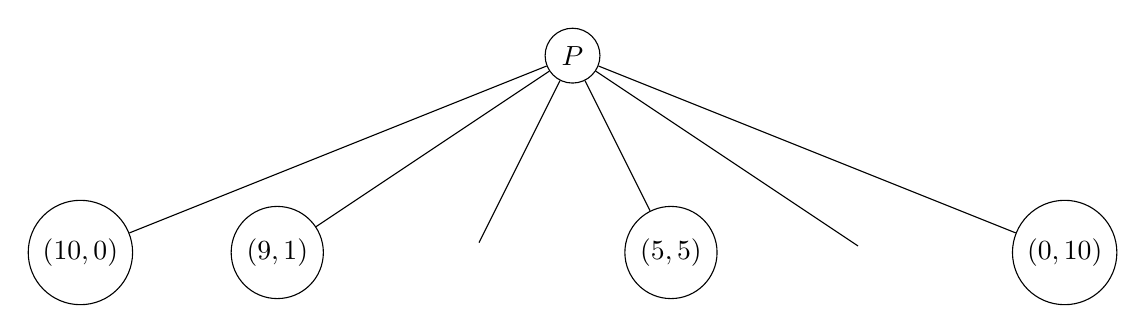
\begin{tikzpicture}[level/.style={sibling distance=25mm/#1}, level 	distance=25mm]
					\node [circle,draw] (z){$P$}
 						child {node [circle,draw] (a) {$(10, 0)$}	}
 						child {node [circle,draw] (b) {$(9, 1)$}	}
 						child {node [] (c) {$ $}	}
 						child {node [circle,draw] (d) {$(5, 5)$}	}
 						child {node [] (e) {$ $}	}
  						child {node [circle,draw] (f) {$(0, 10)$}
					};
					\path (b) -- (c) node [midway] {$\dotsc$};
					\path (c) -- (d) node [midway] {$\dotsc$};
					\path (d) -- (e) node [midway] {$\dotsc$};
					\path (e) -- (f) node [midway] {$\dotsc$};
				\end{tikzpicture}				
			\end{center}
		\item A simple search in the reduced game tree for the strategy with the highest expected payoff for $P$ yields the Sub-Game-Perfect Nash-Equilibrium as we have reached the initial node.
	\end{enumerate}
	$\Rightarrow P$ playing $x_{p} = 10$ together with $R$ always accepting constitutes a Sub-game-Perfect Nash-Equilibrium. 

	Now changing our assumption about player $R$'s decision in case of the offer $0$ leads to
			\begin{itemize}
				\item Again, for $x_{p} \in [0, 10)$ $R$ receives $10 - x_{p} > 0$, therefore he'd have to accept the offer in these situations.
				\item For the remaining offer $0$ ($x_{p} = 10$), it would be just as plausible to refuse the offer, since he is indifferent between both choices. Hence, accepting for $x_{p} \in [0, 10)$ and refusing for $x_{p} = 10$ is also a sub-game perfect strategy.
			\end{itemize}
		 and even if the tree changes only slightly a different Sub-game-Perfect Nash-Equilibrium occurs:
			\begin{center}
				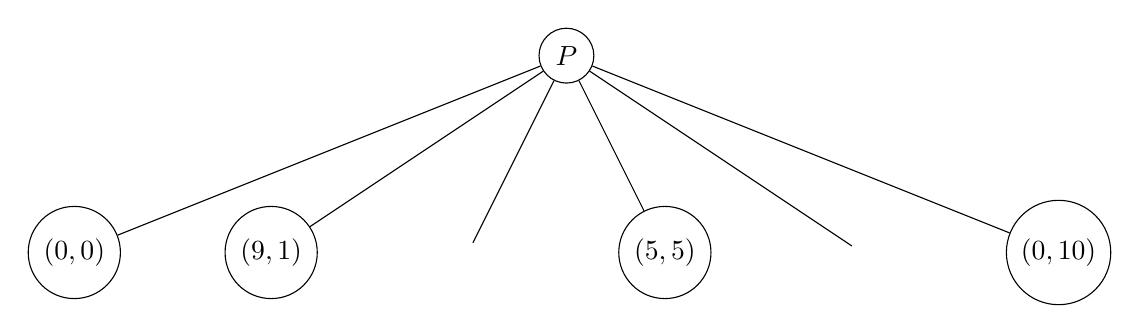
\begin{tikzpicture}[level/.style={sibling distance=25mm/#1}, level 	distance=25mm]
					\node [circle,draw] (z){$P$}
 						child {node [circle,draw] (a) {$(0, 0)$}	}
 						child {node [circle,draw] (b) {$(9, 1)$}	}
 						child {node [] (c) {$ $}	}
 						child {node [circle,draw] (d) {$(5, 5)$}	}
 						child {node [] (e) {$ $}	}
  						child {node [circle,draw] (f) {$(0, 10)$}
					};
					\path (b) -- (c) node [midway] {$\dotsc$};
					\path (c) -- (d) node [midway] {$\dotsc$};
					\path (d) -- (e) node [midway] {$\dotsc$};
					\path (e) -- (f) node [midway] {$\dotsc$};
				\end{tikzpicture}				
			\end{center}
	$\Rightarrow P$ playing $x_{p} = 9$ together with $R$ always accepting if $x_{p} < 10$ and refusing for $x_{p} = 10$ also constitutes a Sub-game-Perfect Nash-Equilibrium. 
\end{example}



\newpage
%!TEX root = Economics and Behaviour.tex

\chapter{How human interactions can change decisions}

\section{An ultimatum game with multidimensional response strategies} 

\begin{itemize}
	\item Güth, W.; Levati, M.V.; Nardi, C.; Soraperra, I. (2014): \textit{An ultimatum game with multidimensional response strategies}. In Jena Economic Research Papers, FriedrichSchiller University and Max Planck Institute of Economics, Jena, Germany (Ultimatum Game)
		\begin{itemize}
			\item We enrich the choice task of responders in ultimatum games by allowing them to independently decide whether to collect what is offered to them and whether to destroy what the proposer demanded. Such a multidimensional response format intends to cast further light on the motives guiding responder behavior. Using a conservative and stringent approach to type classification, we find that the overwhelming majority of responder participants choose consistently with outcomebased preference models. There are, however, few responders that destroy the proposer's demand of a large pie share and concurrently reject their own offer, thereby suggesting a strong concern for integrity.
		\end{itemize}
\end{itemize}
\vspace{-0.5cm}
\section{Cooling Off in Negotiations: Does It Work?}

\begin{itemize}
	\item Oechssler, J.; Roider, A.; Schmitz, P. (2015): Cooling Off in Negotiations: Does it Work?. Journal of Institutional and Theoretical Economics JITE J Inst Theor Econ 171, (2015). (Ultimatum Game)
		\begin{itemize}
			\item Negotiations frequently end in conflict after one party rejects a final offer. In a large-scale Internet experiment, we investigate whether a 24-hour cooling-off period leads to fewer rejections in ultimatum bargaining. We conduct a standard cash treatment and a lottery treatment, where subjects receive lottery tickets for several large prizes. In the lottery treatment, unfair offers are less frequently rejected, and cooling off reduces the rejection rate further. In the cash treatment, rejections are more frequent and remain so after cooling off. We also study the effect of subjects’ degree of “cognitive reflection” on their behaviour.
		\end{itemize}
\end{itemize}
%!TEX root = Economics and Behaviour.tex

\chapter{Level k as a prominent example of a nonstandard/behavioural approach}


\section{Presented papers}

\begin{itemize}
	\item Nagel, R. (1995): \textit{Unraveling in Guessing Games: An Experimental Study}. In: American Economic Review.
		\begin{itemize}
			\item Consider the following game: a large number of players have to state in several rounds simultaneously a number in the closed interval [0, 100]. The winner is the person whose chosen number is closest to the mean of all chosen numbers multiplied by a parameter $p$, where $p$ is common knowledge. The payoff to the winner is a fixed amount, which is independent of the stated number and $p$. If there is a tie, the prize is divided equally among the winners. The other players whose chosen numbers are further away receive nothing.
		\end{itemize}
	\item Müller, J.; Schwieren, C. (2011): \textit{More than Meets the Eye: an Eye-tracking Experiment on the Beauty Contest Game}
		\begin{itemize}
			\item The beauty contest game has been used to analyse how many steps of reasoning subjects are able to perform. A common finding is that a majority seem to have low levels of reasoning. We use eye-tracking to investigate not only the number chosen in the game, but also the strategies in use and the numbers contemplated. We can show that not all cases that are seemingly level-1 or level-2 thinking indeed are – they might be highly sophisticated adaptations to beliefs about other people’s limited reasoning abilities.
		\end{itemize}
\end{itemize}		

\newpage
%!TEX root = Economics and Behaviour.tex


\chapter{Organisations and Markets: The role of market incentives}

\section{Presented papers}

\begin{itemize}
	\item Gneezy, U.; Rustichini, A. (2000): \textit{Pay Enough or Don't Pay at All}. In: Quarterly Journal of Economics.
	\item Gneezy, U.; Rustichini, A. (2000): \textit{A Fine is a Prise}. In: The Journal of Legal Studies. (monetary incentives)
	\item Sebastian Kube, Michel Andre Marechal and Clemens Puppe (2012): \textit{The Currency or Reciprocity: Gift Exchange in the Workplace}. In: American Economics Review. (money versus non-monetary incentives)
	\item Charness, G.; Grieco, D. (2014): \textit{Creativity and Financial Incentives} 
\end{itemize}


\newpage
%!TEX root = Economics and Behaviour.tex

\chapter{Organisations and Markets: The role of moral dimensions of markets}


\section{Morals and Markets}

The possibility that market interactions may erode moral values is a long-standing, but controversial hypothesis in the social sciences, ethic and philosophy. Markets are accused to transform human values in exchange blues and goods into commodities. It has also been argues that market institutions may influence preferences in general with a tendency to make people.

Michael Sandal analysed that with technological progress and the increasing ubiquity of market ideas, since markets continue to enter further and further domains of our social life.

\textit{Further, there is the doux commerce hypothesis, meaning that the entering of market in our social life might improve our situation in many ways...}

\begin{itemize}
	\item Falk, A.; Szech, N. (2013): \textit{Morals and Markets}. In: Science (moral dimensions)
		\begin{itemize}
			\item The possibility that market interaction may erode moral values is a long-standing, but controversial, hypothesis in the social sciences, ethics, and philosophy. To date, empirical evidence on decay of moral values through market interaction has been scarce. We present controlled experimental evidence on how market interaction changes how human subjects value harm and damage done to third parties. In the experiment, subjects decide between either saving the life of a mouse or receiving money. We compare individual decisions to those made in a bilateral and a multilateral market. In both markets, the willingness to kill the mouse is substantially higher than in individual decisions. Furthermore, in the multilateral market, prices for life deteriorate tremendously. In contrast, for morally neutral consumption choices, differences between institutions are small.
		\end{itemize}
\end{itemize}

Examples for market designs where the idea of introducing a free market (money based) is current:
\begin{itemize}
	\item trading markets for emission certificates. To reduce pollution by restricting emission output per country a contract was design, which nevertheless allowed trading of those certificates. M. Sandel was concerned that if we put a money value on pollution it might become less moral concerning to pollute.
	\item Allocation of organs markets: one might be able to trade an incompatible organ for an compatible if available. People started discussing if money should not be introduced in this market instead of just a trading market.
	\item Adoption: high income families might be able to provide better for adopted children and therefore could be preferred on an adoption list
	\item In California child baring is allowed to be traded for money 
\end{itemize}

Restricted markets:

\begin{itemize}
	\item Employment markets are regulated, so exploitation is not (so) present.
\end{itemize}
		
\section{You Owe Me}
\begin{itemize}
	\item Malmendier, U.; Schmidt, K. (2012): \textit{You Owe Me}. In: DOI (moral dimensions)
		\begin{itemize}
			\item In many cultures and industries gifts are given in order to influence the recipient, often at the expense of a third party. Examples include business gifts of firms and lobbyists. In a series of experiments, we show that, even without incentive or informational effects, small gifts strongly influence the recipient’s behaviour in favour of the gift giver, in particular when a third party bears the cost. Subjects are well aware that the gift is given to influence their behaviour but reciprocate nevertheless. Withholding the gift triggers a strong negative response. These findings are inconsistent with the most prominent models of social preferences. We propose an extension of existing theories to capture the observed behaviour by endogenising the “reference group” to whom social preferences are applied. We also show that disclosure and size limits are not effective in reducing the effect of gifts, consistent with our model. Financial incentives ameliorate the effect of the gift but backfire when available but not provided.
		\end{itemize}
\end{itemize}

\section{How Customers' insurance coverage induces sellers' misbehaviour}
\begin{itemize}	
	\item Kerschbamer, R.; Neururer, D.; Sutter, M. (2014): \textit{How Customers' insurance coverage induces sellers' misbehaviour in markets for credence goods}
		\begin{itemize}
			\item Markets for credence goods are characterised by informational asymmetries between expert sellers and their customers, which creates strong incentives for fraudulent behaviour of sellers that results in estimated annual costs to customers and the society as a whole of billions of dollars in the US alone. Prime examples of credence goods are all kinds of repair services, the provision of medical treatments, the sale of software programs, and the provision of taxi rides in unfamiliar cities. In this paper, we examine in a natural field experiment how insurance coverage on the side of the consumer – often prevalent on important markets such as the health care or repair services sectors – can seriously exacerbate inefficiencies in the provision of credence goods by inducing misbehaviour on the side of the seller. Specifically, we study how computer repair shops take advantage of customers’ insurance for repair costs. In a control treatment, the average repair price is about Euro 70, with the repair bill increasing to Euro 129 when the service provider is informed that the insurance would reimburse the bill. Our design allows for a decomposing of the sources of this economically impressive and statistically highly significant difference showing that this is mainly due to the over-provision of parts and overcharging of working time. Overall, our results strongly suggest that insurance coverage greatly increases the extent of misbehaviour of sellers in important sectors of the economy with potentially huge costs to customers and whole economies.
		\end{itemize}
\end{itemize}


\newpage
%!TEX root = Economics and Behaviour.tex


\chapter{Ethics in science}

\section{Pleasures of Skill and Moral Conduct}

Background:
\begin{itemize}
	\item Jeremy Bentham pointed fourteen different $"$simple$"$ sources of pleasures for humans out
	\item In this short list, number three is the $"$pleasure of skill$"$ while number five is $"$the pleasure of a good name$"$.
	\item Yet if being skilful is of crucial importance to people than this can oppose the possibility to keep a good name
\end{itemize}
  
  
  
\textbf{As an example: The Manhattan Project.} After the dropping of the plutonium bomb on Nagasaki, numerous members of the Manhattan Project started worrying about moral implications. Many of the scientists suffered from e.g depressions. \\ 

The Self-Image is so relevant in this concept. Both the desire for mastery and acting in accordance with moral values originate from the same source, a desire for positive self-image. \\ 

The remaining question is therefore: does morality in some (everyday) situations get traded off against skilfulness?


\section{Moral and Markets}

Examples for market designs where the idea of introducing a free market (money based) is current:
\begin{itemize}
	\item trading markets for emission certificates. To reduce pollution by restricting emission output per country a contract was design, which nevertheless allowed trading of those certificates. M. Sandel was concerned that if we put a money value on pollution it might become less moral concerning to pollute.
	\item Allocation of organs markets: one might be able to trade an incompatible organ for an compatible if available. People started discussing if money should not be introduced in this market instead of just a trading market.
	\item Adoption: high income families might be able to provide better for adopted children and therefore could be preferred on an adoption list
	\item In California child baring is allowed to be traded for money 
\end{itemize}

Restricted markets:

\begin{itemize}
	\item Employment markets are regulated, so exploitation is not (so) present.
\end{itemize}



Next, the paper \textit{moral and markets} by Prof. Szech was discussed, issuing the topic:


The possibility that market interactions may erode moral values is a long-standing, but controversial, hypothesis in the social sciences, ethic and philosophy. Markets are accused to transform human values in exchange blues and goods into commodities. It has also been argues that market institutions may influence preferences in general with a tendency to make people.

Michael Sandal analysed that with technological progress and the increasing ubiquity of market ideas, since markets continue to enter further and further domains of our social life.


Further, there is the doux commerce hypothesis, meaning that the entering of market in our social life might improve our situation in many ways...


\section{Presented papers}

\begin{itemize}
	\item Falk, A.; Szech, N. (2016): \textit{Pleasures of Skill and Moral Conduct}. KIT working paper. (non-monetary incentives and morals)
		\begin{itemize}
			\item As was recognised by Bentham, skillfulness is an important source of pleasure. Humans like achievement and to excel in tasks relevant to them. This paper provides controlled experimental evidence that striving for pleasures of skill can have negative moral consequences and causally reduce moral values. In the study, subjects perform an IQ-test. They know that each correctly solved question not only increases test performance but also the likelihood of moral transgression. In terms of self-image, this creates a trade-off between signaling excellence and immoral disposition. We contrast performance in the IQ-test to test scores in an otherwise identical test, which is, however, framed as a simple questionnaire with arguably lower self-relevance. We find that subjects perform significantly better in the IQ-test condition, and thus become more willing to support morally problematic consequences. Willingness to reduce test performance in order to behave more morally is significantly less pronounced in the IQ versus the more neutral context. The findings provide controlled and causal evidence that the desire to succeed in a challenging, self-relevant task has the potential to seduce subjects into immoral behaviours and to significantly decrease values attached to moral outcomes.
		\end{itemize}
	\item Russell, B. (1960): \textit{The Social Responsibilities of Scientists}. In: Science, New Series.
		\begin{itemize}
			\item A scientist can no longer shirk responsibility for the use society makes of his discoveries.
		\end{itemize}
	\item William 0. Baker and more (1961): \textit{The Moral UnNeutrality of Science: The scientist's special responsibility are examined an address given at the 1960 AAAS annual meeting}. In: Science.
		\begin{itemize}
			\item The scientist's special responsibilities are examined in an address given at the 1960 AAAS annual meeting
		\end{itemize}
\end{itemize}


\newpage
%!TEX root = Economics and Behaviour.tex

\chapter{Non-standard utility}


\section{Anticipatory utility}

The standard utility approach states an already deterministic situation on an individuals anticipatable behaviour and this means his utility function is static and can't be changed by additional information. Nevertheless:

\begin{itemize}
	\item Some students decide not to look up their exam grades while on vacation, therefore they refuse gathering free and more important static information to (better) enjoy their free time
	\item Some people with potentially severe diseases avoid getting tested for them.
\end{itemize}

One could argue that even with a bad result they don't have to act upon it, they don't have to behave differently, so why do this situation occur? 

Maybe learning about the future affects well-being today derived from their \textbf{beliefs} about the future.

In Psychology one distinguishes between:
\begin{itemize}
	\item monitors: people who really want to know what is going to happen. E.g. some people want to know every step of their upcoming surgery even though it won't change the outcome
	\item blunders: subjects who don't want the additional information
\end{itemize}

\textbf{Behavioural Economics} by Caplin/Leahy (2001, 2004) tries to combine those two fields

Maybe some people prefer to stick to their Bayesian's priors instead of getting tested because they incorporate their \textbf{beliefs} into their well-being (utility)

~\newline

What if there is an instrumental cost in getting tested?
\begin{itemize}
	\item Caplin/Eliaz (2003): social cost (e.g. HIV tests in america)
	\item Köszegi (2003, 2006): (same as next)
	\item Szech/Schweizer (2015) : individual well-being
\end{itemize}

As solution is propused in both papers the one from Caplin/Eliaz and the one from Szech/Schweizer: coarse tests may be helpful.

~\newline

Maybe sometimes people are able to bias their beliefs away from the Bayesian:
 
Brunnermeier and Parker (2005) and also Oster, Shoulsen, Dorsey (2013) showed that some people might have high risk of inheriting diseases but can convince themselves that the risk is way lower, where this is more then simple optimism. \\



\newpage

\appendix

\cleardoublepage
\phantomsection
\renewcommand{\indexname}{Stichwortverzeichnis}
\addcontentsline{toc}{chapter}{\indexname}
\printindex

\end{document}